\chapter{How Do Developers Learn?}
\label{chapter:learn}

This chapter explores how software developers learn and improve their skills. \autoref{section:how developers learn} introduces the wide range of paths and experiences which contribute to learning, and \autoref{section:document study} describes a study on the inclusion and scope of sustainability teaching for computing students in UK Higher Education

\section**{The Development of Software Skills}
\label{section:how developers learn}

\subsection*{Introduction}

Every decision made is based on a large number of factors, many of which have been accumulated prior to the making of the actual decision \citep{Zeleny1982}. A complete examination of the prior experience and knowledge which informs every software development decision is beyond the scope of this research. However, there are some key sources of learning common to many developers.

Self-study is a common way into software development. In the early days of home computing, learning was often from magazines or other commercial publications \citep{Thegreatone9982021} but with the growth of the web and the proliferation of open source software it is now common for new programmers to learn by looking at other code and searching for examples or tutorials on the web. One effect of this form of self-study is that it is very much based on finding code examples which are similar enough to the desired solution, and then tinkering until things seem to work. While this can be a quick and effective way to create code to solve specific problems, its effectiveness as a learning tool is questionable. Developers who have learned to code using this copy-and-tweak approach can find it difficult to design larger solutions or work on more complex projects with other developers.

Learning software development with peer support is a way to address some of its issues. When functioning well, peer support can help new coders develop and express their understanding and provide prompts for exploring other possibilities \citep{Boud1999}. Peer-based learning has its drawbacks, though. For example, it can be hard for the knowledge and understanding of the group members to exceed the knowledge and understanding of the most knowledgeable in the group. If nobody has encountered a concept or technique it is unlikely to arise in discussion, and misunderstandings shared in the group are as likely to be spread as truths \citep{Herrmann-Werner2017}.

For people starting software development later in life, there are may routes into employment \citep{Hyrynsalmi2024}. In such cases, training often comes from an employer or from a vendor-sponsored training or certification program, targeted at specific tasks or roles, or at the use of specific products, but may also include more general aspects of the field. 

A classic route into a software development career is through an undergraduate computing course of some kind. Undergraduate study of computing, considering specifically the inclusion and scope of sustainability topics in UK computing courses, is explored in more detail in \autoref{section:document study}.

\subsection*{Problems with Experiential Learning}

A mixture of on-the-job learning, self-study, and peer learning can be very flexible, and has the advantage of being much more closely suited to the needs of working in a particular position on a particular application than any more general educational curriculum. However it is not universally positive. A needs-driven, ad-hoc method of learning can lead to a variety of software problems, many of which are common in real-world software projects.

An employer wants to get value from every new employee, and for software developers that usually means working on real software as soon as possible. While some organisations are large enough and reflective enough to have good support networks in place, many simply put a new hire to work on the assumption that he or she already has all the skills needed. This approach can be highly motivational for learning, but may require using techniques and tools which are not fully understood. More experienced and cynical software developers often recommend that an initial attempt at solving a software problem should be treated as a draft or a rehearsal for the real thing \citep{Brooks1995}, but for a developer who lacks that experience it can easily seem that as soon as it seems to work, it is `good enough'. With this approach, large code-bases can grow to include a lot of such na{\"\i}ve solutions, which can in turn lead to bigger problems later.

The presence of sub-optimal code in an application would not be a problem if the code were to be continually improved, as such sections would soon be removed or updated. Unfortunately, this is rarely the case, as everyone on the project is too busy either creating new code or fixing more visible problems. As a code-base grows it also becomes increasingly hard for anyone to understand the whole application and the subtleties of the interaction between all the various parts. Making changes without deep understanding could result in introducing more problems than it solves. This in turn leads to an attitude of `if it ain't broke, don't fix it', where poor code remains in the system, potentially forever. Sometimes, the pressure to add new features as quickly and cheaply as possible means that poor code will even be copied and re-used elsewhere in the application. This prevalence of code of unknown quality makes it tricky for learners to gain the most from working with it, and can propagate misconceptions and poor choices.

The continual accumulation of poor code and quick fixes is common enough to have been given the name `technical debt'. Traditionally, the only way to `pay off' this debt would be to completely rewrite the application \citep{Brooks1995} but this is not always financially feasible. A range of techniques and approaches have been developed to recognise such \emph{code smells} \citep{Sharma2017}, retroactively improve code quality through \emph{refactoring} \citep{Fowler1999}, and to develop code which is better structured and easier to understand in the first place, such as \emph{test-driven development} \citep{Beck2022}.

Once a team has produced code for an application, that code has a weight of precedence, and it becomes harder to deviate from the existing design and coding approaches. This historical bias can also hinder learners who might be unaware of the difference between, or are unable to judge between, local traditions and alternative approaches. Where third-party components are used in a system, the same effect can be seen. It can appear easier and more effective to re-use a component which has already been included in a project than to explore the possibility that there might be an alternative which is more suitable. This force is particularly strong where a vendor of something important (and probably expensive), such as the computer hardware, operating system, application platform, or database, endorses some components. A decision to stick with a vendor-approved option will almost always seem easier and better than evaluating, and learning from, something new and untried.

All on-the-job learning, by its nature, takes place in the context and pressures of work. Sometimes there will be a conflict between the immediate needs of the job, and the longer-term goal of learning the skills to do the job better. This is a difficult conflict to resolve, and the decision often falls in favour of the urgent rather than the long-term value of learning. Where an organisation does set aside time and money for training it is often arranged by people with no direct experience of the needs of the individuals concerned, and may be provided more for other reasons such as regulatory compliance than for genuine learning.

The pressures of learning while at work lead many software developers to study and practice their skills while `off the clock'. This can potentially be much more effective than trying to fit in learning around doing a job, but has challenges of its own. Such personal learning can conflict with family, social, or personal well-being responsibilities, but also faces more insidious problems. Many people find it easier to learn and develop their skills on personal projects which have little or nothing to do with work. Employers, however, often make claims over any intellectual property created by employees whether `at work' or not, and are wary of any employee who engages in peer-learning outside the organisation for fear that they might somehow `leak' important information.

\subsection*{The Inclusion of Sustainability}

This research is about sustainability and the environmental impact of software, so it's natural to wonder where learning about sustainability might fit in all the ways described above that software developers learn their craft and skills. The answer is complex, and depends on where you look.

Personal projects, peer-learning, and on-the-job experience are difficult to quantify, as the experience of each person is so different. What can be seen in these forms of learning is that they are generally driven by the need in the moment, and therefore concentrate more on finding answers to solve specific problems than on a broader approach to study. A typical method of learning in these situations will involve finding a source of examples, which might be a general web search, a specific community site such as Stack Overflow\footnote{\url{https://stackoverflow.com/}}, or a body of shared code within an organisation. Whether or not such code examples emphasise, or even acknowledge, sustainability issues is more difficult to determine. Personal experience suggests that many such examples ignore this aspect of software development responsibility in favour of more \emph{functional} concerns. This ease and speed of access to solutions or components to resolve immediate problems can often mean that \emph{non-functional} issues such as sustainability are sidelined.

Formal learning through corporate and vendor training, schools, apprenticeships, and universities should be able to provide a broader and more nuanced education, particularly for courses which follow guidelines or seek accreditation from professional bodies. While there are signs that guidelines for such courses are increasingly including environmental, ethical, and sustainability concerns in their guidance, the practical impact of this guidance depends on the uptake by the teaching establishments.

The next section explores one aspect of software developer learning in more detail with a study of the inclusion of sustainability topics in United Kingdom Higher Education computing curricula.

\section*{Sustainability Teaching in UK Higher Education}
\label{section:document study}

\subsection*{Introduction}

Education is in a unique position as it has the opportunity to inform now and direct for decades to come. The purpose of education is a contentious area, but this study will use a definition from the OECD: \enquote{to equip learners with the knowledge, skills, attitudes, and values that they will need for their future} \citep{Schleicher2018}. Graduates can then use such knowledge, skills, attitudes, and values to shape the world they live in. This future world will require understanding of sustainability and its challenges.  

Education for sustainability is clearly important, but within educational  literature there is little consensus on either the meaning and scope of sustainability or whether and how to teach it. \citet{Abernethy2014} noted that many institutional initiatives go little further than local campus practices such as a recycling program. In a Spanish study, sustainable use of resources had a lower priority than social and cultural sustainability \citep{Sanchez-Carracedo2021}. \citet{Shephard2013} found that individual ideas about sustainability varied widely among teaching staff and this influenced their teaching.

Sustainability education may also have different impact in different personal and career paths. All students, regardless of future career, would arguably benefit from education which prepares them to \enquote{find solutions to the pressing problems of the day} \citep{Shephard2013} including sustainability. \citet{Junger2024} took a stronger view, stating \enquote{Implementing aspects of sustainability, such as Green Coding techniques, into the training of future IT professionals is a crucial step to bringing sustainability into view for software producers while providing them with a workforce capable of implementing sustainability into their development process}. \citet{Cotton2013} discovered that university students have a greater commitment to environmental sustainability than the general population. Some graduates, however, might achieve the potential for a larger impact, for example those whose future includes responsibility for political policies, influencing large organisations, or developing products and services used by millions (or even billions) of people. When designing sustainability education, it is therefore important to consider the potential benefits of the teaching throughout the future lives of the students.

One way to model the value of such teaching is to estimate and compare the potential sustainability impact across multiple areas. There are many approaches to such modelling, and a full investigation of this topic is beyond the scope of this study. Consideration will be limited to the potential impact on greenhouse gas (GHG) emissions for three representative scopes of sustainability education:

\begin{itemize}
    \item \textbf{Scope 1: Personal and lifestyle sustainability} Each person contributes a certain amount of GHG each year but this differs based on their location and lifestyle. In the UK, figures range widely but commonly quoted examples include 6.26 tonnes \citep{GlobalChangeDataLab2021} or 10-13 tonnes \citep{Campbell2022}. Much of this contribution, however, is incurred collectively, largely out of the control of the individual. Whatever the actual GHG contribution, there is a hard limit to the potential gains just from personal lifestyle improvements. 
    \item \textbf{Scope 2: Institution and infrastructure sustainability} The operation of a typical educational institution contributes between thousands and hundreds of thousands of tonnes \citep{Helmers2021}. Education which helps reduce this could have a larger impact but as the sustainability of the institution improves each contributor faces diminishing returns.
    \item \textbf{Scope 3: Subject and career-specific sustainability} The potential gains in this area are several orders of magnitude greater than personal sustainability. \citet{Griffin2017} points out that just 100 companies are responsible for 71\% of the world's GHG emissions. Even minor improvements in one of these contexts could be hugely important globally. Major policy changes or sustainability improvements to a product or service used daily by millions of people could have similarly large benefits.
\end{itemize}

Scopes 1 and 2 have the advantage that they are immediately applicable and suitable for all students. The impact of Scope 3 will usually be delayed at least until a student has graduated and found a situation where they can use what they have learned. All of the above scopes are worthwhile and will need to be addressed in time. However, human society need to reduce GHG emissions as much as possible, as soon as possible, so it would make sense to prioritise the largest, as well as quickest, gains. Therefore, society need graduates who have the knowledge, skills, attitudes and values to make a difference in high-impact career areas as well as their personal and educational lives.

\begin{figure}[ht]
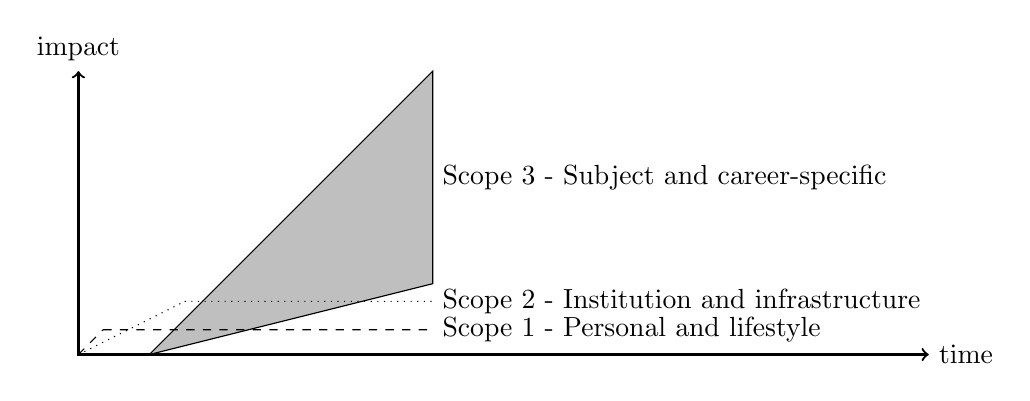
\begin{tikzpicture}[scale=0.9]
    % axes
    \draw [<->,thick] (0,4) node [anchor=south] {impact}
        |- (12,0) node [anchor=west] {time};
    % data
    \draw (5,2.5) node [anchor=west] {Scope 3 - Subject and career-specific};
    \draw [fill=lightgray] (1,0) -- (5,4) -- (5,1) -- cycle;
    \draw [dashed] (0,0) -- (0.35,0.35) (0.35,0.35) -- (5,0.35) node [anchor=west] {Scope 1 - Personal and lifestyle};
    \draw [dotted] (0,0) -- (1.5,0.75) (1.5,0.75) -- (5,0.75) node [anchor=west] {Scope 2 - Institution and infrastructure};
\end{tikzpicture}
\caption{\label{impact-image}Estimated potential global impact over time}
\end{figure}

As discussed in \autoref{section:intro about}, Information and communication technology (ICT) is an example of a potentially high-impact career sector. Practitioners in such areas need to learn the craft of their future profession, and the most common source for this is higher education (HE). The 2022 annual Stack Overflow Developer Survey \citep{StackOverflow2022} found that around 90\% of the 70,000 software developers sampled had attended a university or other HE institution. However, that survey does not break down the responses by discipline or major and sampling software developers is notoriously difficult \citep{Baltes2016}.  Computing is widely viewed as a degree with  plentiful jobs and good salaries, so it is reasonable to assume that although the computing profession is not exclusive to computing graduates, most graduates of computing programmes spend at least some time in computing jobs and therefore HE computing education provides key input to work performance. 

The climate crisis and the huge environmental impact of computer systems has elevated sustainability to the status of a \emph{Threshold Concept} \citep{Rodger2015} \citep{Cousin2006} and has led to research into how to incorporate sustainability in computing courses. Attempts have largely taken one of three \citep{Pattinson2011} approaches: a standalone course, module, or elective on sustainability \citep{Penzenstadler2011a} \citep{Penzenstadler2018} \citep{Cai2010}; integrating sustainability into existing courses and modules \citep{Abernethy2014} \citep{Mishra2021}, or setting project-based work with sustainability aspects \citep{Jaccheri2021} \citep{KaskeJr2022}. Some researchers have argued that sustainability should be included as part of ethics \citep{Ozkaya2019}, \citep{Moraga2017}, \citep{Bednar2020}. Unlike more research-based disciplines, ethics in computing is almost exclusively concerned with the potential future uses and abuses of technology \citep{Alidoosti2022}.

In the United Kingdom, the Quality Assurance Agency for Higher Education (QAA) oversees educational standards but there is no central HE curriculum. The QAA provides guidelines for education on sustainable development \citep{QAA2021} but these are not discipline specific and individual institutions are responsible for designing their own curricula based on these guidelines. The British Computer Society (BCS) also offers accreditation for computing courses in the United Kingdom and the Commonwealth. The BCS guidelines include \enquote{environmental and sustainability aspects} among several \enquote{external factors which may affect the work of the computer professional} \citep{BCS2022}.  Including a topic in accreditation guidelines, however, does not automatically imply that it is being taught. \citet{Torre2017} surveyed 33 academics from 13 different countries who had expressed an interest in `green' computing but found that, even within this group, \enquote{sustainability is under-represented in the curricula}. \citet{Malik2019} investigated the inclusion of sustainability in computing education in Pakistan and found that \enquote{the curriculum is yet to incorporate the essential aspects of sustainability into its programs and courses.} \citet{Sanchez-Carracedo2021} examined the inclusion of sustainability in education courses at a Spanish university and also found that \enquote{much remains to be done in the academic field to fully incorporate sustainability into higher education.}  It is not clear how much and in what form sustainability has been included in current UK HE computing courses.

The following sections introduce the research questions which drove this research, then consider the process used to gather results and analyse the different kinds of findings. Results and their implications will be discussed, and limitations and future work explored before finally drawing some conclusions.

\subsection*{Methods}

\subsubsection*{Research Questions and Study Structure}

This study addressed two initial research questions:
\begin{itemize}
\item \textbf{RQ1}: To what extent is sustainability teaching included in UK Higher Education computing courses?
\item \textbf{RQ2}: In courses which contain sustainability teaching, what is the scope of that teaching?
\end{itemize}

A mixed-methods approach was used, structured in two phases. One phase was primarily quantitative, collecting and analysing numerical data to address RQ1. The other phase was primarily qualitative, examining email responses and curriculum documents to understand the approach taken in sustainability teaching by each course and its course team.

During the study, a third, less-formal, question arose: 
\begin{itemize}
\item \textbf{RQ3}: How much detail is publicly available about UK HE computing courses?
\end{itemize}
This question was explored as a side-effect of the data collection for RQ1.

\subsubsection*{Process}

To evaluate the inclusion of sustainability in UK Higher Education (HE) computing curricula, The names and web URLs of all UK HE institutions offering computing-related courses were collected. The institution websites were searched for general information on their approach to sustainability. In cases where insufficient information was available on the websites, an appropriate course leader was identified and sent an email requesting information about the inclusion of sustainability in their courses. Finally, the email responses and any curriculum documents which had been obtained were analysed.

Institutions and individuals are anonymised in this study. Details found by a web search are indicated with a \textbf{W} Prefix (e.g. W1) and details found in email responses are indicated with a \textbf{R} prefix.

\newcommand{\funnelsection}[3]{
    \path[name path=line1] (0,#1)--(10,#1);
    \path [name intersections={of = left and line1}];
    \coordinate (A)  at (intersection-1);
    \path [name intersections={of = right and line1}];
    \coordinate (B)  at (intersection-1);
    \draw [dashed] (A) -- (B) node [align=center, midway, below] {#2};%
}
\begin{figure}[ht]
\centering
\begin{tikzpicture}
    % funnel body
    \draw [name path=left] (0.5,9) -- (4.5,2) (4.5,2) -- (4.5,1);
    \draw [name path=right] (9.5,9) -- (5.5,2) (5.5,2) -- (5.5,1);

    % funnel sections
    \funnelsection{9}{Collect Institutions} \\
    \funnelsection{8}{Examine Websites} \\
    \funnelsection{7}{Find Course Leaders} \\
    \funnelsection{6}{Send Emails} \\
    \funnelsection{5}{Re-send Emails} \\
    \funnelsection{4}{Analyse\\ Responses} \\
    \funnelsection{3}{} \\

    % collection tray
    \draw [thick] (0,2) -- (0,0) (0,0) -- (10,0) (10, 0) -- (10, 2);
    \draw [dashed] (0,0.5) -- (10,0.5) node [midway, below] {Curriculum Details};

    % web spout
    \path[dotted, name path=bottom] (0,7)--(10,7);
    \path [name intersections={of = bottom and left}];
    \coordinate (A)  at (intersection-1);
    \clip (A) -- (0.5,7) -- (0.5,9) --cycle;
    \draw[name path=outer] (1.5,7) circle (0.75);
    \draw[name path=inner] (1.5,7) circle (0.35);
\end{tikzpicture}
\caption{\label{funnel-image}Document acquisition funnel}
\end{figure}

To determine which institutions to include in the study, A manual search was performed on the course listing pages at the UCAS website \citep{UCAS2020}. By selecting only undergraduate courses and the starting year, with no other search keywords, this provided a full list of available undergraduate courses in the UK. From that list was selected all universities which offer at least one course in computing, computer science, software engineering or a small number of other equivalent courses. Joint courses such as computing with business or specialist courses such as creative computing, cybersecurity, or computer games design were not included. 109 separate UK HE institutions offering computing courses were identified. This shows that computing is a popular discipline for both institutions and undergraduates.

The websites were also examined for information about the environment and sustainability priorities of the institution. Where available, the provided site search facility was used to search for `sustainability'. Results were excluded from specific courses or modules, and any transient information such as blog posts, news items or case studies. For most institutions this led to at least one page describing their position on sustainability. In a few cases this search did not turn up anything useful, so page headers, footers, and links were examined to look for the same thing. By the end of this phase of the search a sustainability page or policy document had been identified for 97 of the 109 institutions.

Each of these sustainability pages were examined each in turn to determine how they mapped to the three sustainability scopes for this study. This process was to some degree subjective, as the pages and documents had little in common by way of structure or organisation. 

To determine which courses or departments were accredited by any professional accrediting bodies the course pages and department pages for each course and institution were inspected to determine which ones contained either an accreditation logo or equivalent text such as `accredited by the BCS'. 86 of the 109 institutions in the study claimed BCS accreditation. This is roughly 79\%, indicating that accreditation is a priority for most institutions. No courses claimed accreditation by other bodies such as the ACM.

In an initial attempt to find course curricula for computing courses at these institutions, each website was examined by site search (if provided) and by following internal links. The aim was to locate publicly available curricula for these courses. It quickly became apparent that information on UK HE websites does not generally contain enough information to determine whether teaching on sustainability is included. Only one institution (W1) provided and linked a publicly available course handbook. A typical course web page consisted of a brief introduction and a list of mandatory and optional modules, each with only a short description. No courses were identified which contained any explicit content on sustainability, and where sustainability was mentioned it was in general terms about the sustainability of the institution and the teaching approach (scope 2).

To gain access to sustainability content of the courses staff were contacted directly. Each university website was searched again, this time looking for contact details for course leaders or department heads with curriculum responsibility for computing courses. It was a lengthy process, but eventually uncovered an email address at each of the remaining 108 institutions. An email was drafted and sent to each of the email addresses. Each email provoked one of four classes of result: no response at all, an automated response indicating that the recipient was temporarily or permanently unavailable, a manual response indicating that the recipient no longer had responsibility in that area, or a personal response. In cases where an alternative email address was provided, the same email was sent to the new address. 

To cope with cases of temporary absence or email problems, the same email was re-sent after a delay of a few months to any recipients who had not responded at all. There were no additional responses to this second wave, so no further emails were sent.

Within the information which was available, there were further problems including a conflict of terminology between disciplines. The field of software engineering uses some of the keywords with very different meanings. In this field, \emph{sustainability} has traditionally been aligned with \emph{maintainability} -- the ability of a computer system to remain in useful operation over time \citep{Venters2021} and there continues to be disagreement on the meaning of the term \citep{Venters2014}. Likewise, the word \emph{environment} also has many different meanings. In software terms, an environment describes the configuration for a particular instance of a system. The word \emph{environment} also often appears in educational documents in senses such as \enquote{a supportive environment} or \enquote{Virtual Learning Environment}. In this study, such clashes of terminology led to some false positive matches which were investigated and then excluded.

\subsection*{Results}

\subsubsection*{Institutional Positions}

All of the 97 institution sustainability documents indicated at least something about scope 2 (institution and infrastructure) but considerably fewer mentioned scope 1 (personal and lifestyle) or scope 3 (subject and career-specific) sustainability. [\autoref{ring-chart1}]. The emphasis on other aspects of sustainability varied widely. Themes common to many institutions included the declaration of a `climate emergency', a discussion of the UN sustainability goals (see \autoref{section:un goals}), and highlighting the favourable position of the institution in one of the many local, national, and global environmental and sustainability ranking schemes.

\begin{figure}
\newcommand{\coloursector}[5]{%
  \fill[#5] (#1:#3) arc[start angle=#1, end angle=#2, radius=#3] -- (#2:#4) arc[start angle=#2, end angle=#1, radius=#4] -- cycle;
}
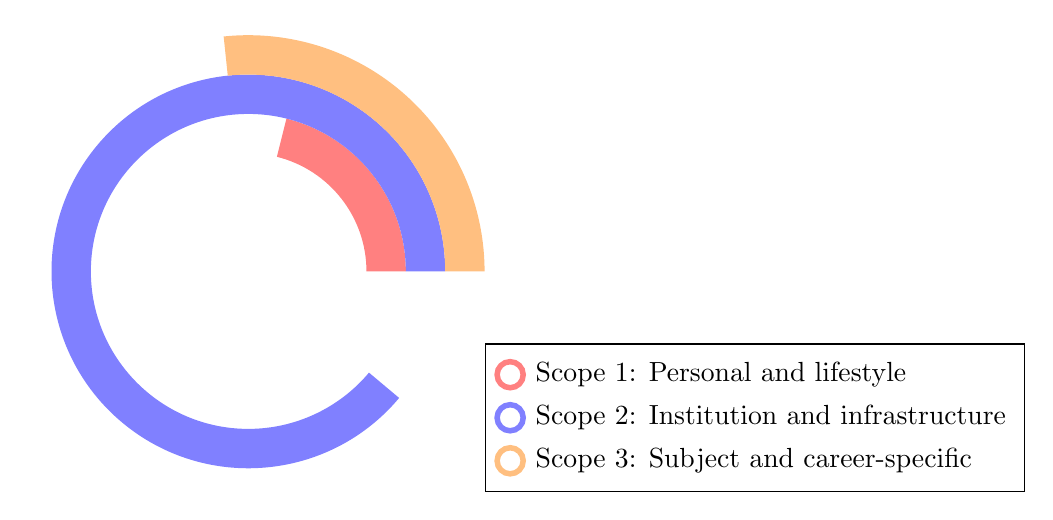
\begin{tikzpicture} [
  scale=0.5,
  rednode/.style={shape=circle, draw=red!50, line width=2},
  bluenode/.style={shape=circle, draw=blue!50, line width=2},
  orangenode/.style={shape=circle, draw=orange!50, line width=2}
]
\coloursector{0}{76}{3}{4}{red!50!white}
\coloursector{0}{320}{4}{5}{blue!50!white}
\coloursector{0}{96}{5}{6}{orange!50!white}
\matrix [anchor=south west, draw] at (current bounding box.south east) {
  \node [rednode,label=right:Scope 1: Personal and lifestyle] {}; \\
  \node [bluenode,label=right:Scope 2: Institution and infrastructure] {}; \\
  \node [orangenode,label=right:Scope 3: Subject and career-specific] {}; \\
};
\end{tikzpicture}
\caption{\label{ring-chart1}Sustainability priorities as a proportion of surveyed institutions}
\end{figure}

\subsubsection*{Responses}

In total, ignoring the unproductive second wave, 112 emails were sent and 22 responses received, of which 11 were personal responses [\autoref{responses-table}]. The other 11 responses either redirected to a colleague or abnegated responsibility and have been excluded from further analysis. The remaining responses map to five categories [\autoref{categories-table}].

\begin{table}
\begin{tabular}{ll}
\toprule
Response & Description \\
\midrule
W1 & Full course handbook found using website search.\\
R1 & Provided a link to a course handbook.\\
R2 & Provided a link to a detailed course outline and some discussion. \\
R3 & Provided a link to a course outline and a comment about an archived course. \\
R4 & Provided a general link to the university website.  \\
R5 & Replied recommending the university website. \\
R6 & Replied '\emph{I am unable to release such documents.}'  \\
R7 & Replied with attached documents.  \\
R8 & Replied with a course outline and a discussion.  \\
R9 & Provided a link to a course outline.  \\
R10 & Replied with a discussion.  \\
R11 & Replied with a discussion.  \\
\bottomrule \\
\end{tabular}
\caption{\label{responses-table}Summary of informational responses.}
\end{table}

\begin{table}
\begin{tabular}{lr} \toprule
Category & Responses \\
\midrule
Refusal & R6 \\
Link to the university website & R4, R5 \\
Discussion & R2, R3, R8, R10, R11 \\
Course outline or overview & R2, R3, R8, R9 \\
Curriculum documents as a link or an attachment & W1, R1, R7, (R9) \\
\bottomrule \\
\end{tabular}
\caption{\label{categories-table}Response categories.}
\end{table}

Eliminating responses with a refusal or just a link to the university website leaves eight meaningful responses to analyse spread across three categories.

\subsubsection*{Analysis of Discussion Responses}

\textbf{Respondent R2} replied with the URL of some curriculum documents for a MEng course and a BSc course, both in Computer Science. R2 commented:
\begin{quote}
    The second-year core unit Interaction and Society has some elements of sustainability, I believe.
\end{quote}
In addition, R2 noted that all students at their institution have access to an online course named \emph{Unleash Your Potential: Sustainable Futures} hosted by FutureLearn \citep{Preist2020}. This course appears to consist of guidance on generally living a sustainable life (scope 1).

\textbf{Respondent R3} replied with link to a general course outline but also noted that they previously provided a module on \emph{Environment and Sustainability} to all students of engineering and computing in 2017-2018, but this module is no longer offered to computing students.

\textbf{Respondent R8} replied with a link to a course outline and also commented:
\begin{quote}
    I don’t know if sustainability is incorporated in any modules. Although I think there were plans to include sustainability topics in the MSc titled: Programme and project management MSc, which you can also access from the above link. There is definitely some need to think about this topic from energy demand perspectives as big data processing requires a lot of energy especially in the area of crypto currency where data centres are sometimes turned off to save energy.
\end{quote}

\textbf{Respondent R10} provided links to several modules included in computing courses, and also noted:
\begin{quote}
    Sustainability questions, broadly understood, are covered in a number of our compulsory modules, even if this term is not used that explicitly in our module specifications.
\end{quote}

\textbf{Respondent R11} did not provide any course links, but instead commented:
\begin{quote}
    This is a topic close to my heart, but I'm afraid the answer is rather disappointing.  I don't believe sustainability is taught in our programme at all (other than third year projects I and some of my colleagues run on energy/thermal comfort and related topics).  I am pushing for it's inclusion as part of our ongoing curriculum review.
    
    If your topic is beyond the UK, then I know there are good programmes at KTH (Daniel Pargman, Elina Eriksson), and probably Toronto (Tomlinson).  The sustainable HCI google group might be a way to do this - the CPHC list may also be good for UK visibility for your request.
    
    This may well change institutionally as part of our recent climate emergency declaration.
\end{quote}

\subsubsection*{Analysis of Course Outlines}

The course outlines provided by \textbf{Respondent R2} included links to module descriptions for all mandatory and optional modules on each course. The module indicated in the discussion (\emph{Interaction and Society}) made no explicit mention of sustainability, but did include the following paragraph:
\begin{quote}
    The second half of this unit focuses on computer scientists in society. We will consider both how individuals, groups, societies, and environments are impacted by digital technologies, and on the role and responsibilities of computer scientists. We will introduce approaches to consider impacts, drawing on theories of ethics, values, responsible innovation, and social computing.
\end{quote}

None of the course and module links provided by \textbf{Respondent R3} contained any explicit mention of sustainability. Module information was mostly limited to the name of the module or a few sentences of description. The course materials referenced by \textbf{Respondent R8} also contained no explicit mention of sustainability and were similarly brief. The course and module links provided by \textbf{Respondent R9} provided more detail than the other respondents in this category, and the course details included a link to a detailed program specification document. 

\subsubsection*{Analysis of Curriculum Documents}

The curriculum documents found using a web search (\textbf{W1}) contain no mention of sustainability, environmental impact or energy use, although there is a blanket statement that:
\begin{quote}
    On each level of your course you will learn about social, legal and ethical aspects of Computing, which will broaden your understanding of the way the world works and how communication and collaboration are evolving.
\end{quote}

\textbf{Respondent R1} included a link to a course handbook, but the link was invalid. It appeared that the website had been re-organised without maintaining old links. The supplied link did include a course code in the URL, so it required some further searching to find the correct location. The curriculum documents provided by this respondent include the following statement:
\begin{quote}
    This undergraduate computing degree aims to equip students with key competencies to analyse complex problems, and design, implement and evaluate innovative, ethical and sustainable digital solutions to a wide range of problems in modern society.
\end{quote}
The terms `sustainability' and `environment' appeared several times in the course overview, but there was no further information about the content of specific modules.

The curriculum documents provided by \textbf{Respondent R7} are comprehensive and informative. Learning outcomes for each of the provided programmes are mapped to the UN Sustainability goals and sustainability is mentioned in various forms in both mandatory and optional modules. Among the educational aims and learning outcomes it suggests teaching for scope 3, stating:
\begin{quote}
    To develop graduates who are able to understand the current and future capabilities of computer-based information systems as resources and can creatively and innovatively deliver technical computing solutions, engaging developers and technical development teams to deliver required outcomes in ethical and sustainable ways.
\end{quote}

The curriculum document indirectly provided by \textbf{Respondent R9} contains no mention of sustainability or the environmental or social impact of software, despite claims that the aim of the course is:
\begin{quote}
To produce graduates who are technical experts, but who also have an
awareness of the business, social, legal and ethical contexts of IT.
\end{quote}

\subsubsection*{Application to Research Questions}

\subsubsubsection{RQ1}

Despite the high proportion of institutions which expressed a strong position on the environment and sustainability [\autoref{ring-chart1}], no public evidence of the inclusion of sustainability teaching in computing courses was found. Full examination of curricula for other disciplines was beyond the scope of this study, but several examples and case studies of sustainability teaching in other disciplines was noticed while looking for institution sustainability policies. This indicates that institutions are willing to share such cases when they have them, which lends further weight to the argument that these are lacking in computing.

The small number of email responses, and the potential skew towards respondents who had something they were proud to share, reduces the contribution of the email responses to RQ1, but there was evidence of sustainability teaching in four responses [\autoref{RQ1-inclusion}], which indicates that there is at least some teaching of sustainability in computing, even though it is not visible in public course details.

\begin{table}
\begin{tabular}{lrrrrr} \toprule
 & Considered & Responded & Curriculum & Sustainability \\
\midrule
Website & 109 & & 1 & 0 \\
Email & 108 & 22 & 8 & 4 \\
\midrule
Totals & \textbf{109} & & \textbf{9} & \textbf{4} \\
\bottomrule \\
\end{tabular}
\caption{\label{RQ1-inclusion} RQ1: Sustainability inclusion in curricula}
\end{table}

\subsubsubsection{RQ2}

The lack of public information about computing course curricula and the general lack of inclusion of sustainability in available course materials made it difficult to address RQ2. The information which was obtained appears to mirror the literature in often conflating the various scopes and impacts of sustainability into a single broad topic. Where specific aspects of sustainability are mentioned it is often in very general terms, possibly because these are easier to apply as a policy across the institution regardless of discipline.

Of the course details analyzed, only a small proportion mentioned sustainability or environmental issues in any form, and of those which did, the emphasis was often unspecified, with just two providing clear enough information to establish the scope of the teaching and only one of those being the potentially high-impact scope 3. Subject-specific teaching must also be considered in the context of any institution-wide programmes which are primarily scope 1 and scope 2.

\begin{table}
\begin{tabular}{lccccc} \toprule & \multicolumn{4}{l}{Sustainability Scope} \\
\cmidrule{2-6}
Response & S1 & S2 & S3 & Unspecified & None\\
\midrule
 W1 & & & & & \checkmark \\
 R1 & & & & \checkmark & \\
 R2 & \checkmark & & & & \\
 R3 & & & & & \checkmark \\
 R7 & & & \checkmark & & \\
 R8 & & & & & \checkmark \\
 R9 & & & & & \checkmark \\
 R10 & & & & \checkmark & \\
 R11 & & & & & \checkmark \\
\bottomrule \\
\end{tabular}
\caption{\label{RQ2-scopes} RQ2: Sustainability scopes in available curricula}
\end{table}

\subsubsubsection{RQ3}

It became increasingly clear that the educational institution websites which were studied had largely been set up to function as an online version of a traditional printed prospectus, with no more detail than could be fitted onto a page or two per course. There is almost certainly much more information available internally, but it is not made easy for prospective students and other interested parties to access. There were also problems with broken internal links on websites showing that things had been changed and moved around without checking the consistency of the website.

A third problem with institution websites was the surprising difficulty of finding staff names, responsibilities and research interests. On many websites such information was not included in the provided `site search', and often not even available by following links via departments or courses. In some cases the only option was a single huge staff directory, usually ordered by surname, which required a laborious process of stepping though looking for appropriate departmental and course responsibilities. In some cases this information was also incorrect or out-of-date.

\subsection*{Discussion}

\subsubsection*{Content}

The website survey results show that sustainability is clearly a priority for the majority of HE institutions which teach computing courses. This stands in stark contrast to the small amount of subject-specific teaching which was available for this potentially high impact discipline. Where sustainability education was available there was a tendency to include it either as a separate discipline in its own right or defer it to Masters-level study. According to the Stack Overflow developer survey \citep{StackOverflow2022} only around 25\% of the developers surveyed had studied to postgraduate level in any discipline. It seems reasonable to assume that relatively few developers will have completed such a Masters computing course or graduated from a specific course in the environment or sustainability. For sustainability teaching to have an impact on the work of software developers it needs to be included as a core topic in the university and college courses which educate the majority of professional software developers.

However, there are major issues with including any new topic into a curriculum \citep{Annala2017} and computing is already crowded. Employers, and therefore students, demand immediately-applicable skills such as experience with specific computer systems, programming languages and technologies. The landscape of these skills and technologies is continually expanding, and every new addition puts more pressure on existing courses \citep{Vessey2005}. Course teams need to continually learn and update teaching in order to stay relevant. The vocational nature of computing, and its potential for high-earning employment, often leads to large class sizes which in turn implies a heavy marking and support load for already busy lecturers. This leaves less time and energy for research and consideration of the implications of the teaching.

In UK HE, every course is required to be \emph{validated} before it may be delivered to students. Validation is not only required for the creation of new courses but also for any substantive changes. This is often viewed as a cumbersome process to be avoided or put off where possible. While this may be a sensible strategy for disciplines which change relatively slowly, it acts to create a great deal of tension in fast-moving areas such as technology and the environment. Some course teams deliberately choose to describe curricula in loose terms allowing lecturers to adapt courses or include more topical material without requiring curriculum changes and re-validation. My institution, for example, currently includes sustainability and environmental impact in software engineering topics about cloud computing and cryptocurrencies, but such aspects are not mentioned on the website or in the public prospectus.

This `under the radar' approach may have contributed to the dearth of publicly available course curricula on institutional websites. While this approach can help to keep courses fresh without the burden of re-validation, it makes it very difficult for prospective students to determine what is \emph{actually} included in the teaching before committing to a choice of institution and course of study. We live in an internet age and an institution website is almost always the first port of call for anyone interested in study or research collaboration. An institutional website needs to provide more than just a prospectus of short course summaries. UK HE institutions need to reconsider this vital part of their public appearance.

There is also potentially an issue with the interpretation of terminology such as `sustainable' and `environment' which are used to mean different things in different disciplines. If policymakers and those responsible for implementing the policies have different understandings of the same language, then the result is unlikely to be what the policymakers envision. This could be a contributing factor in the lack of sustainability teaching even in cases where the institution as a whole has strong sustainability goals or where the topic has been picked up more eagerly in other disciplines.

Although outside the scope of this research, there were clues both on institution websites and in email responses that sustainability teaching may be taken more seriously in other subject areas. Environmental science courses are an obvious example, but there were also some mentions of sustainability in engineering, architecture and some business courses. This indicates that the inclusion of sustainability topics varies not only by institution but also by discipline.

\subsubsection*{Context}

This study was limited to HE institutions in the UK, and is therefore indicative only of the state of computing education in the UK. The British tradition of HE has several key characteristics which informed the results of this study. Individual institutions are broadly free to design and deliver their own courses subject to validation, as discussed above, and any guidelines from the QAA and independent bodies such as the BCS. There is a naming and classification system \citep{UCAS2018}, which provides some assistance when looking for courses, but within each category, courses vary widely and can include or emphasise whichever topics each course team feels are appropriate. Prospective students apply for a small number of courses, usually at different institutions, and each student's scheme of study is fully defined by the course which they eventually attend. Typically in computing courses most modules are mandatory for all students with some choice offered between a small set of options in later years. Generalisations are tricky, though, as each institution can define the path through each of their courses.

While it might be possible to generalise or draw parallels with the situation in other countries, it is important to note that other nations and other cultures have different HE traditions \citep{UNESCO2023}, but it is not common to declare this context. Much of the literature in this field appears to come from what one might call the `American' tradition. In this tradition, students apply to an institution but then may choose from a wide range of individual classes from many disciplines before eventually declaring a major. Each different major may require some specific classes or offer a suggested plan of study in order to graduate, but students may still gain credit for other classes, such as additional classes in sustainability, if they wish. On the other hand, \citet{Malik2019} situated their study in what one might call the `Islamic' tradition. Culture and education are more closely tied in this tradition, and there is often greater central oversight on course contents. This enabled \citeauthor{Malik2019} to examine a single curriculum document and apply their conclusions to the whole of Pakistan, an approach which would not work in the UK. Any study of educational content therefore needs to be situated in the context of its national and cultural traditions.

\subsubsection*{Limitations and Future Research}

There are several potential limitations to this study. The first is the small sample size. Any conclusions are specific to the particular responses and documents which were analysed, and therefore might be skewed by or biased to those respondents and courses. It is clear that most institutions consider sustainability to be a priority, but there are no results from the study on which to base conclusions about \emph{why} most institutions failed to make curriculum information available on their websites, or why many staff members who were contacted declined to respond.

The scope of this study is also a potential limitation. Only UK HE institutions listed in the UCAS search system \citep{UCAS2020} and which offered at least one course with one of a small set of names were included. Any institutions or courses which did not match these criteria have not been considered. There may be, for example, some private institutions \citep{Hunt2023}, or courses which are only offered to students associated with a particular sponsoring organisation \citep{TheScholarshipHub2023}, which might refute the conclusions. However, such institutions and courses form a small proportion of the overall UK HE sector and the majority of prospective students look to the UCAS system when choosing an institution and course of study.

This study highlighted several areas worthy of future research. More study is needed on current trends in university websites, and how well they suit the needs of prospective and current students as well as researchers and other interested parties. Further study is also needed on how students select courses in such complex and technical areas as computing, particularly when there is so little detail available. Additional research would be useful on how lecturers and other course team members deal with important areas which are not explicitly mentioned in curriculum documents, and how that is shared with students. The most important area for further work, though is distinguishing and mapping the different scopes of sustainability education and exploring the theory that the kinds of sustainability topics, approaches, and skills being taught should adapt to the discipline of study and the potential sustainability impact of graduate career paths.

\subsection*{UK HE Study Conclusions}

The intention of this study was to determine the extent to which sustainability education is included in UK HE computing courses (RQ1) and the scope of that education (RQ2). A general lack of detailed information shared on university websites forced a switch to contacting individual course leaders to ask directly for information about their courses. Only a small number of responses were received, but within those responses the answer to RQ1 was clear -- very few institutions include explicit sustainability teaching in computing, even when the institution as a whole has a strong posture on sustainability or claims course accreditation by bodies which require it. The lack of detailed information for RQ1 made it difficult to answer RQ2, but there were some indications which generally agree with the literature that most sustainability teaching in HE is unspecific, or aimed at local or personal sustainability rather than teaching students how to use their subject knowledge and skills to address the big issues of the future.

In conclusion, UK HE institutions appear to be failing in their obligations to inform prospective students of what they will study, and to prepare the next generation of computing professionals for the current climate sustainability crisis. 

\section*{Overall Learning Discussion}

There are many different routes into the software development industry and each individual learns their skills in different ways. A major industry survey indicated that a large proportion of software developers have had a college or university education but, in the UK at least, there is little evidence of the inclusion of sustainability teaching in undergraduate computing courses. This is despite increasing awareness of global sustainability issues and pressure from accrediting bodies. The contribution of computing systems to the ongoing climate emergency is very large, but it seems unlikely that new software developers will be ready to tackle this task without a major shift in emphasis in computing education.

If the education process is not providing a flow of software developers and other decision-makers skilled in sustainable computing, then other approaches are needed. One such approach is to develop and promote information and tools to assist in integrating sustainability in the existing software development process. \autoref{chapter:performance} investigates comparing the efficiency of software components in order to minimise the computing hardware, and its associated energy use, needed for some common large-scale problems. \autoref{chapter:testrig} develops a low-cost apparatus for the direct comparison of software energy use when selecting software or during the development of software applications. \autoref{chapter:intermediate} and \autoref{chapter:comp energy} develop further software tools and use the comparison apparatus to compare the energy usage of the software components investigated in earlier chapters.

\subsection*{The State of Sustainable Computing Teaching in UK HE}
\label{contrib:HE}

When considering media attention, the requirements of accrediting bodies, and institution publicity, it is easy to assume that Higher Education computing courses are preparing the next generation of software developers and other decision makers to address the ongoing climate emergency and the huge contribution of computing systems to greenhouse gas emissions.

This research has shown that, in the UK at least, this is not yet the case. Courses claim accreditation based on older standards which do not include sustainability clauses, and those institutions which do include sustainability teaching tend to favour personal and institutional sustainability advice such as campus waste recycling programs and remembering to switch off room lighting. Even where teaching staff are aware of bigger issues, it has often proved difficult to fit computing system sustainability topics into an already crowded curriculum.

